\subsection{Validation} \label{s:N_II:validation}

The point of this section is to show that the changes made were seen in the network.


\subsubsection{Network metrics}

\begin{itemize}
    \item How are the network metrics compared between the standard and reward of the non-tumour?
    \item But between standard network in tumour and standard in non-tumour?
    \item What are the genes difference?
\end{itemize}

To study the differences between the non-tumour and tumour networks the previously used graph metrics (degree, pageRank, closeness, betwenees and IVI)\footnote{Reminder: the degree - node's number of connections; pageRank - node's centrality; closeness - how close the nodes are; betwenees - nodes between; IVI - a combination of network metrics} are shown in \cref{fig:N_II:net_metrics_comp}. There are four networks compared, the standard (red) and reward (green) for tumour derived, and the correspodant for non-tumour (mustdard - standard and blue - reward).

% Degreee & PageRank
In the pageRank and degree metrics, the non-tumour networks seems to be elongated on the Y-axis, denoting a a high variance between the nodes. This is further enforced by the reward modifier, suggesting that there is a subset of nodes that have a high number of connections and are central to the network. Compared to the non-tumour, the TCGA derived graphs have nodes that are more similar in their centrality and the number of connections. The tumour networks having similar values for centrality and degree. 

% Closeness & betweneess
A distinct feature of the tumour networks is that there the there are a subset of genes that are close together given by the closeness plot. The reward non-tumour network has the nodes closer compared with the standard, indicating the reward modifier 'brings' the node closer. Another distinct feature of the tumour networks is that the two networks genes with high betenees values. Again, the reward modifier amplifies this compared to the standard (this is not very clear).

% IVI
The IVI distribution for the two tumour networks are largely similar, but there is a noticeable between the non-tumour standard and reward graphs. It can be seen that the when the weight modifier is applied, the distribution is sparser, havig a subset of genes that have higher values.

Overall the metrics comparisons shows that the non-tumour network react stronger to the reward modifiers and that there is a subset of genes that are more central and have a large number of connections.





\begin{figure}[!htb]    
    \centering
    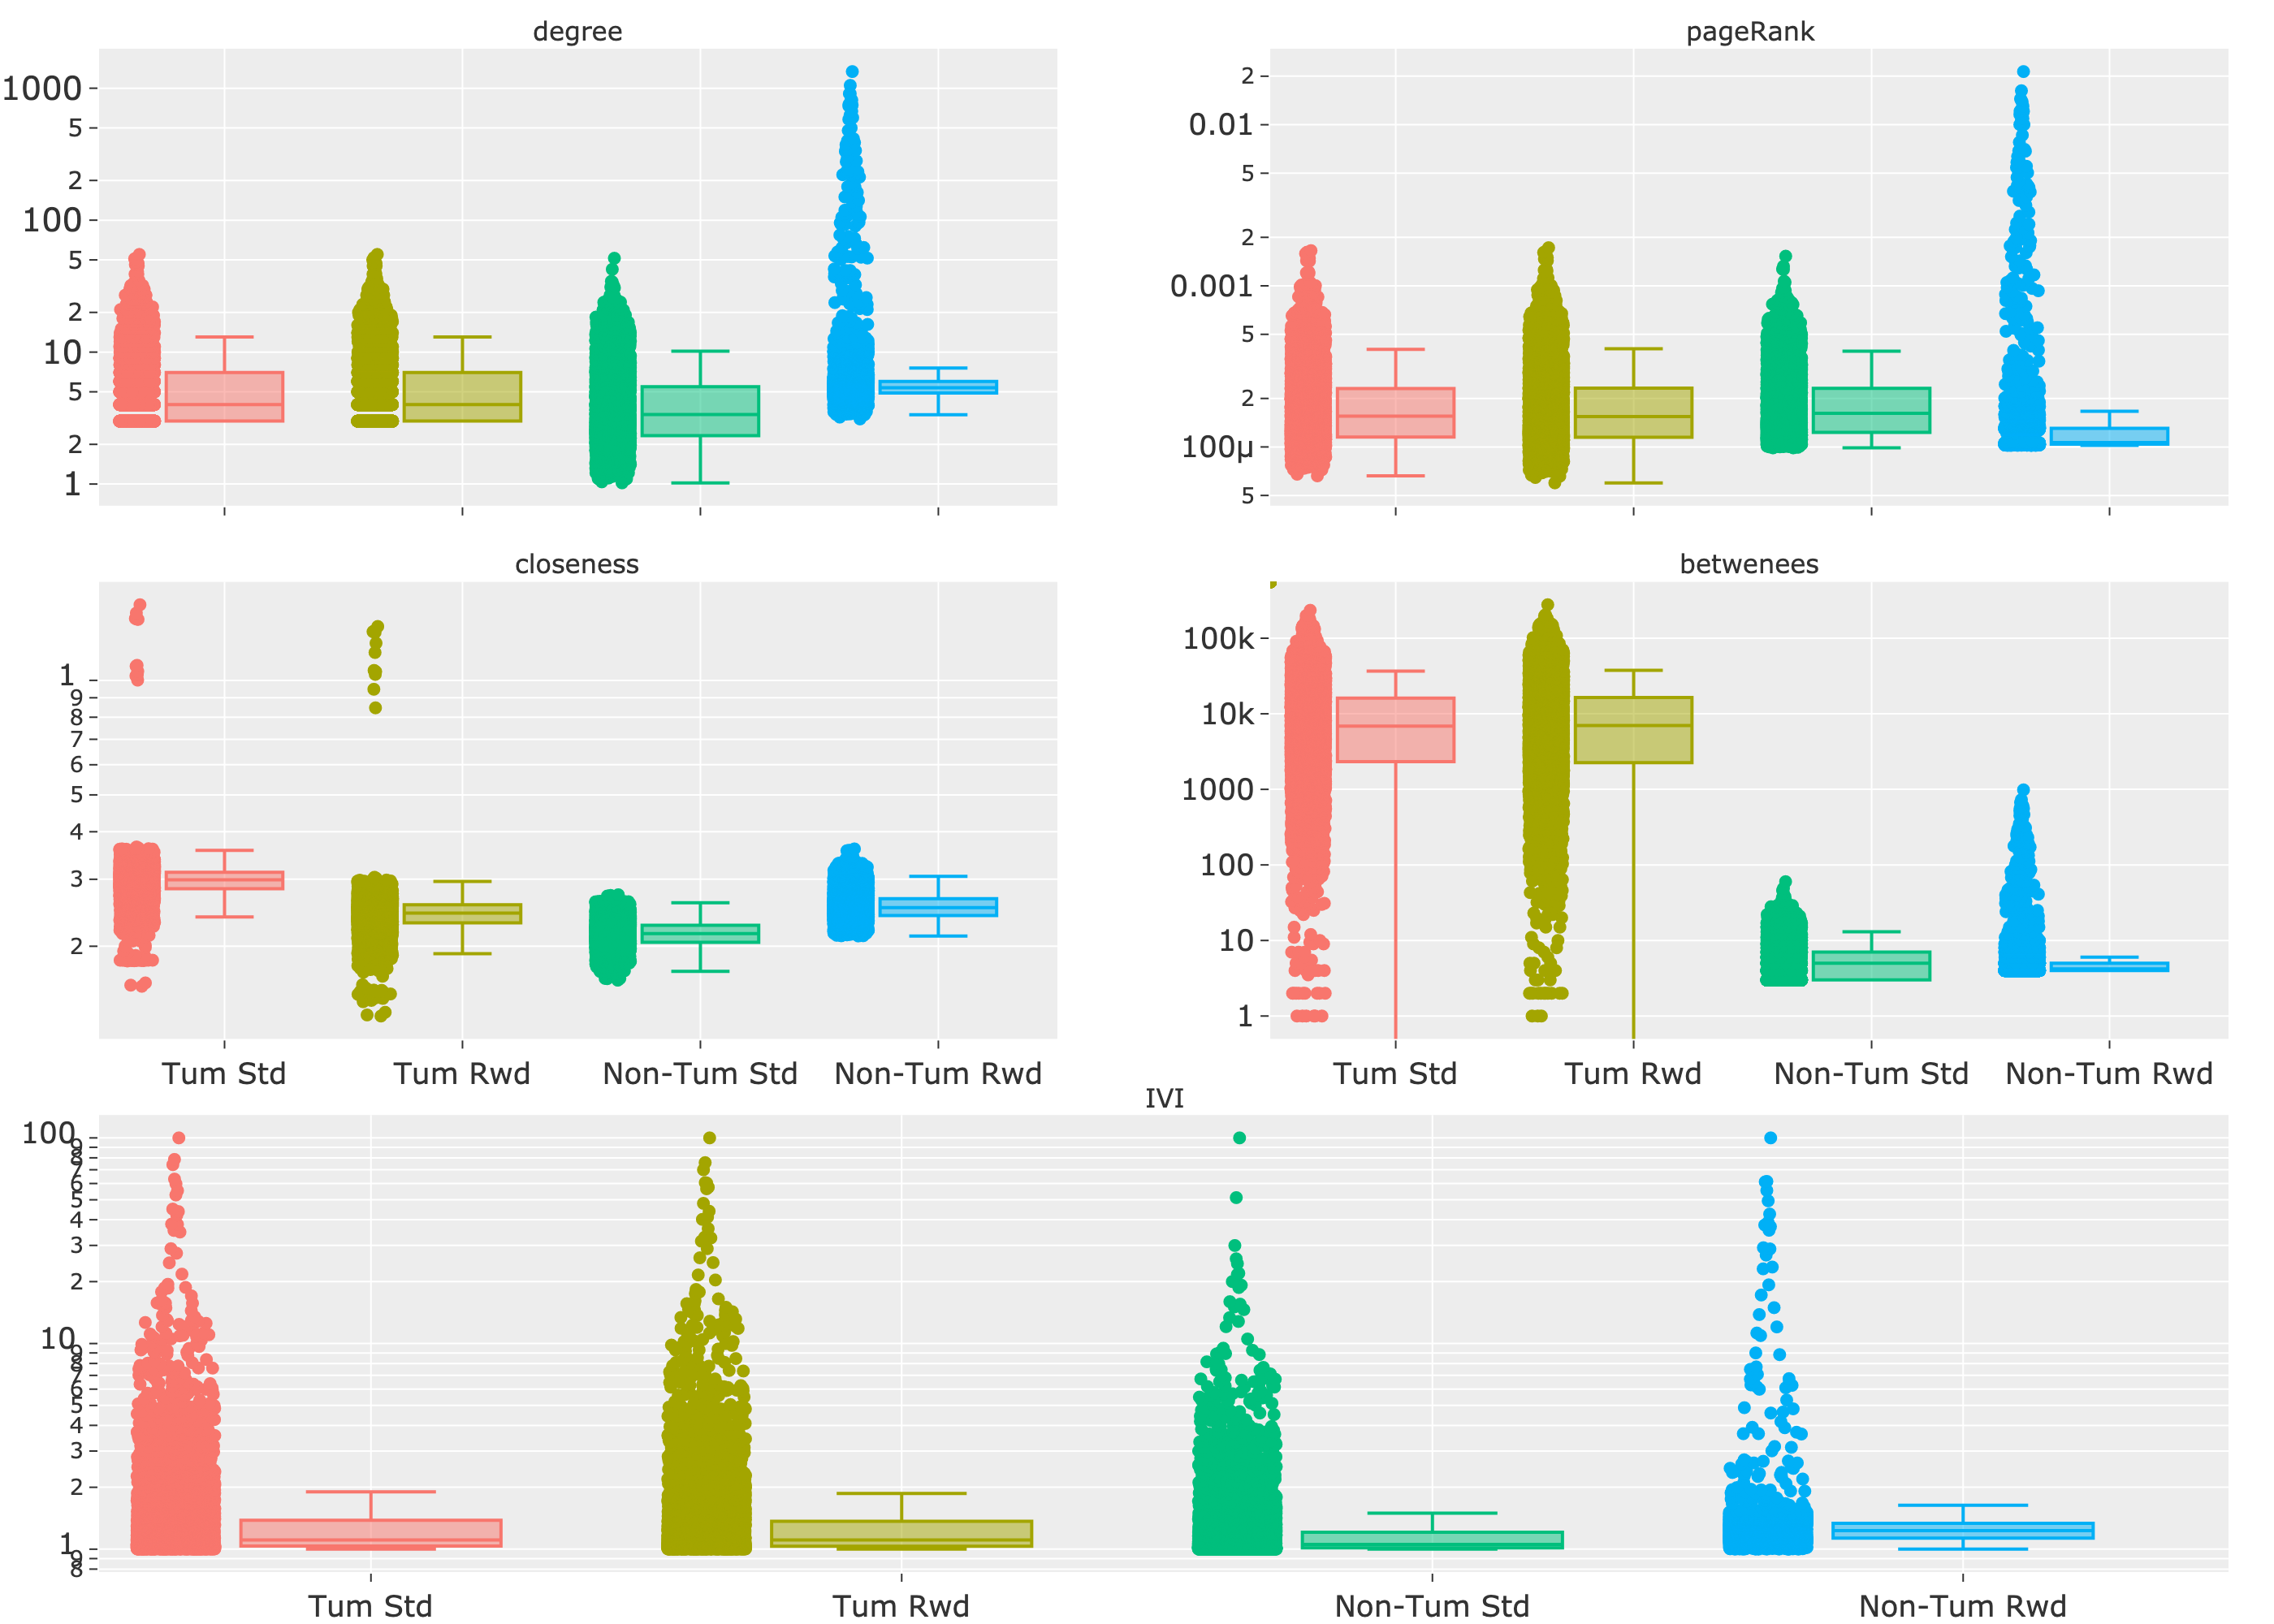
\includegraphics[width=1.0\textwidth,height=0.7\textheight,keepaspectratio]{Sections/Network_II/validation/network_comparison.png}
    \caption{Network metrics for the Tumour and non-tumour networks with no modifier and reward modifier. The y-axis represent the log10 of the metric. }
    \label{fig:N_II:net_metrics_comp}
\end{figure}



\subsubsection{Standard and Reward comparison}

\subsubsection{Community detection}

\subsubsection{Tumour network vs Non-tumour network}

How can we measure this change?